% Szglab4
% ===========================================================================
%
\chapter{Analízis modell kidolgozása 2}

\thispagestyle{fancy}

\section{Objektum katalógus}

\subsection{Enemy}
Az \textbf{Enemy} osztály példányai egy-egy ellenséget tárolnak. Rendelkeznek típussal (fajjal), pillanatnyi pozícióval, hátralévő életerővel. Az idő haladtával próbálnak végighaladni egy véletlenszerűen választott lehetséges útvonalon.

\subsection{EnemyType}
Leírja egy ellenségtípus (jelen esetben a négy faj: ember, tünde, törp vagy hobbit) tulajdonságait, mint például az alapsebessége és a kezdeti életereje. Minden ellenségnek van egy referenciája egy példányára, amely meghatározza a viselkedését.

\subsection{Game}
Ez a játék logikáját magába foglaló osztály. Számon tartja a pályán lévő ellenfeleket, akadályokat és tornyokat, valamint végrehajtja a kiválasztott misszió által leírt forgatókönyvet, ami alapján az ellenségek érkeznek.

\subsection{Gem}
Egy épületekre rakható varázskő tulajdonságait tárolja. A \textbf{Game} osztály fog példányokat létrehozni belőle, különböző tulajdonságokkal. Ha egy épületre rá van rakva egy fajta varázskő, akkor az épület egy referenciát tárol a példányára.

\subsection{Map}
A \textbf{Map} a pályát képviseli, melyben N darab \textbf{Waypoint} van. A pálya egy külső fájlból betölthető, ami új játék indulásakor fog megtörténni, miután kiválasztja a játékos a pályát. A pálya különböző tulajdonságai is lekérdezhetőek, amelyek ahhoz kellenek, hogy meg lehessen allapítani, hogy lehet-e oda új tornyot/akadályt építeni.

\subsection{Mission}
Egy \textbf{Mission} objektumban lesz eltárolva, hogy milyen ellenségek, mikor és honnan jönnek be a pályára. Ez a három adat majd egy segéd osztályban lesz összefogva, és egy tárolóban lesz tárolva. A játék főciklusa le tudja majd kérdezni a következő ellenséget, melyet az objektum visszaad, ha már elég idő eltelt az előző egység óta (ha nem akkor nem ad vissza egységet).

\subsection{Obstacle}
Egy akadályt valósít meg. Ha egy ellenség belelép egy olyan mezőbe, amin van egy \textbf{Obstacle}, akkor azt egy bizonyos mértékben lelassítja, az ellenség fajától függően.

\subsection{ObstacleGem}
Egy akadályokra rakható varázskő tulajdonságait tárolja, a \textbf{Gem} leszármazottja. A \textbf{Gem} tulajdonságain kívül olyan tulajdonságokat is módosíthat, ami csak az akadályoknak van.

\subsection{Projectile}
Ez az osztály egy lövedék leírása. Amikor egy torony lő, akkor példányosítja ezt az osztályt a cél ellenség átadásával, így egy lövedék mindig a torony által meghatározott ellenség után megy, amit ha megfelelően megközelít (eltalálja az ellenséget), akkor levesz az életerejéből és megsemmisíti magát.

\subsection{Waypoint}
A \textbf{Waypoint}-ok kitűznek egy útvonalat, amelyen az ellenségek menni fognak. El van tárolva bennük a pozíciójuk, a távolságuk a céltól, valamint a következő \textbf{Waypoint} ahova az út folytatódik. Ezek mind le is kérdezhetőek.

\subsection{Tower}
Egy tornyot valósít meg. Ha egy ellenség a hatókörébe ér, akkor elindít egy \textbf{Projectile}-t az irányába, a tüzelési gyakoriságának megfelelő időközönként. Ha több ellenfél van a hatókörében, akkor arra lő, aki a legközelebb van a célhoz.

\subsection{TowerGem}
Egy tornyokra rakható varázskő tulajdonságait tárolja, a \textbf{Gem} leszármazottja. A \textbf{Gem} tulajdonságain kívül olyan tulajdonságokat is módosíthat, ami csak a tornyoknak van.


\section{Statikus struktúra diagramok}

\begin{figure}[H]
\begin{center}
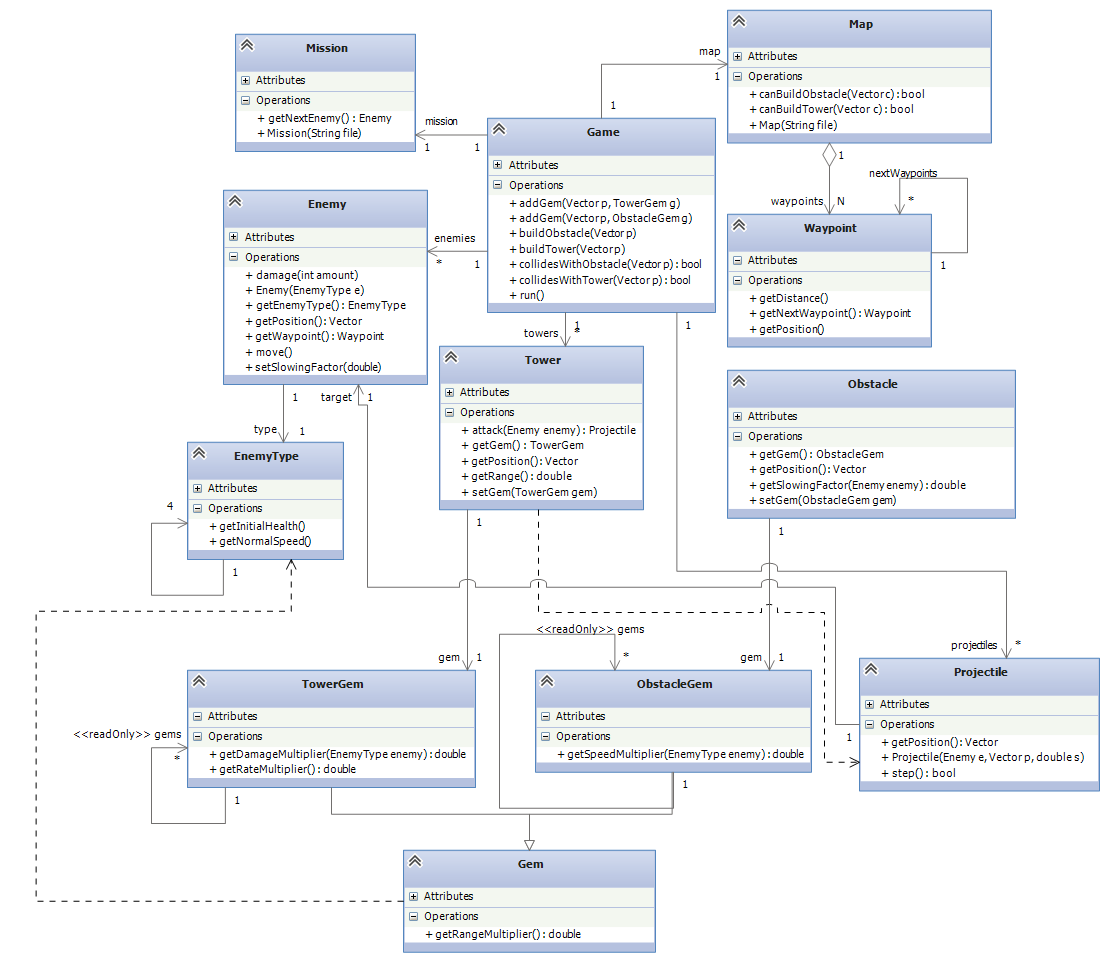
\includegraphics[width=177mm]{images/ch04/class.png}
\caption{Osztálydiagram}
\label{fig:class_diag}
\end{center}
\end{figure}


\section{Osztályok leírása}


\subsection{Enemy}
\begin{itemize}
\item Felelősség\\
Az ellenségek pozíciójának, sebességének és életerejének nyilvántartása.
\item Attribútumok
	\begin{itemize}
		\item \textbf{EnemyType} type: Az egység típusa.
		\item double health: Az ellenség fennmaradó életereje.
		\item \textbf{Vector} position: Pillanatnyi pozíció a pályán.
		\item \textbf{Waypoint} targetWaypoint: Az a \textbf{Waypoint}, ami felé az ellenség jelenleg tart.
		\item double slowingFactor: Az \textbf{EnemyType} sebességét ezzel kell beszorozni, hogy megkapjuk az ellenség tényleges jelenlegi sebességét.
	\end{itemize}
\item Metódusok
	\begin{itemize}
		\item Enemy(EnemyType et, Waypoint start): Létrehoz egy et typusú \textbf{Enemy}-t a start \textbf{Waypoint}-helyén.
		\item boolean move(): Az ellenséget a sebességének megfelelő mértékben mozgatja a célja irányába. Ha az ellenség életereje 0 vagy kisebb, akkor true-val tér visza, egyébként false-al.
		\item boolean damage(double amount): Csökkenti az ellenség életerejét amount-al, igazzal tér vissza ha az ellenség meghalt.
		\item \textbf{Vector} getPosition(): A position attribútum értékével tér vissza.
		\item \textbf{EnemyType} getEnemyType(): Visszaadja az ellenség típusát.
		\item double getDistance(): Visszaadja az ellenség céltól való távolságát a legrövidebb úton haladva.
		\item void setSlowingFactor(double sf): Beállítja a slowingFactor-t sf-re.
	\end{itemize}
\end{itemize}


\subsection{EnemyType}
\begin{itemize}
\item Felelősség\\
Leírja egy bizonyos típusú (fajú) ellenség alapvető tulajdonságait. Egy-egy példányára hivatkozik az összes ellenség, amelyeknek ezáltal meghatározza a viselkedését.
\item Attribútumok
	\begin{itemize}
		\item int cost: Az ilyen fajtájú ellenségek ára varázserőben.
		\item double initialHealth: Az ilyen fajtájú ellenségek kezdeti életereje.
		\item double normalSpeed: Az ilyen fajtájú ellenségek akadályoztatás nélküli haladási sebessége.
	\end{itemize}
\item Metódusok
	\begin{itemize}
		\item double getInitialHealth(): Visszaadja az initialHealth attribútum értékét.
		\item double getNormalSpeed(): Visszaadja a normalSpeed attribútum értékét.
	\end{itemize}
\end{itemize}




\subsection{Game}
\begin{itemize}
\item Felelősség\\
A többi osztály nyilván tartása és összekötése, a játékbeli események vezérlése. A felhasználói felülettől érkező parancsok végrehajtása, és a játék állapotának rendelkezésre bocsájtása a kijelzéshez.
\item Attribútumok
	\begin{itemize}
		\item \textbf{ArrayList}<\textbf{Projectile}> projectiles: Eltárolja a jelenleg játékban lévő lövedékeket.
		\item \textbf{Map} map: Referencia a kiválasztott pályára, amin a játék folyik.
		\item \textbf{Mission} mission: Referencia a kiválasztott misszióra, amely alapján zajlik a játék.
		\item \textbf{ArrayList}<\textbf{Building}> buildings: Eltárolja a játékos megépített tornyait.
		\item \textbf{ArrayList}<\textbf{Gem}> gems: Az összes lehetséges, toronyra illetve akadályra rakható varázskő nyilvántartása.
		\item \textbf{ArrayList}<\textbf{EnemyType}> types: Ez a lehetséges ellenségtípusok listája.
		\item \textbf{ArrayList}<\textbf{Enemy}> enemies: Az összes éppen látható ellenség található meg benne.
		\item int magic: A játékos jelenlegi varázsereje.
	\end{itemize}
\item Metódusok
	\begin{itemize}
		\item void run(): Ez a metódus futtatja a főciklust, amelyben maga a játék működik.
		\item void buildTower(\textbf{Vector} position): Épít egy tornyot a paraméterül kapott helyen évő mezőre.
		\item void buildObstacle(\textbf{Vector} position): Épít egy akadályt a paraméterül kapott helyen lévő mezőre.
		\item void addGem(\textbf{Vector} position, \textbf{Gem} gem): A paraméterként kapott helyen lévő toronyra vagy akadályra rárakja a paraméterként kapott varázskövet.
	\end{itemize}
\end{itemize}




\subsection{Gem}
\begin{itemize}
\item Felelősség\\
Egy általános varázskő tulajdonságainak tárolása.
\item Attribútumok
	\begin{itemize}
		\item int cost: A varázskő ára varázserőben.
		\item double rangeMultiplier: Megadja, hogy a varázskővel ellátott toronynak hányszorosára nő a hatótávolsága.
	\end{itemize}
\item Metódusok
	\begin{itemize}
		\item double getRangeMultiplier(): Visszaadja a varázskő hatótávolság szorzóját.
	\end{itemize}
\end{itemize}


\subsection{Map}
\begin{itemize}
\item Felelősség\\
Tartlamaz az összes \textbf{Waypoint} referenciát, felelős a kapott fájlból beolvasni a pályát, és felépíteni azt, valamint meg kell mondja, hogy van-e út a megadott \textbf{Vector}-nál.
\item Attribútumok
	\begin{itemize}
		\item List <\textbf{Waypoint}> waypoints: A pályán található \textbf{Waypoint}-ok listája.
	\end{itemize}
\item Metódusok
	\begin{itemize}
		\item bool canBuildObstacle(\textbf{Vector}): A \textbf{Waypoint}-ok alapján visszaadja, hogy lehet-e akadályt építeni a megadott helyen.
		\item bool canBuildTower(\textbf{Vector}): A \textbf{Waypoint}-ok alapján visszaadja, hogy lehet-e tornyot építeni a megadott helyen.
		\item Map(\textbf{String} file): Betölti a kapott elérési útvonalon a fájlt, és felépíti az alapján a pályát.
	\end{itemize}
\end{itemize}


\subsection{Mission}
\begin{itemize}
\item Felelősség\\
Felelőssége, felépíteni a listát, amely a beérkező ellenségeket és időzítésüket tartalmazza. Majd a megfelelő időközönként ki kell adja ezeket az egységeket a \textbf{Game} osztálynak.
\item Attribútumok
	\begin{itemize}
		\item \textbf{List}<\textbf{Spawn}> spawnList: A Spawn segédosztályban tárolt ellenség-idő-belépési pont, adatokat tárolja.
		\item double lastSpawn: Tárolja az előző spawn idejét.
	\end{itemize}
\item Metódusok
	\begin{itemize}
		\item \textbf{Enemy} getNextEnemy(double time): A spawnList listaból a következő elemet megvizsgaálja, és ha spawnolni kell a következő ellenséget, akkor visszaadja azt.
		\item Mission(\textbf{String} file): Betölti a kapott elérési útvonalon a fájlt, és felépíti az alapján a listát (spawnList).
	\end{itemize}
\end{itemize}


\subsection{Obstacle}
\begin{itemize}
\item Felelősség\\
Felelős, az ellenfelek lassításáért, úgy, hogy meg kell tudnia mondani a pozícióját, valamint, hogy az adott ellenséget mennyire lassítja.
\item Attribútumok
	\begin{itemize}
		\item \underline{int cost}: Az akadály ára varázserőben.
		\item \textbf{Gem} gem: Eltárol egy referenciát egy \textbf{Gem} típusú objektumra, ami meghatározza, hogy az adott épület milyen echant alatt áll.
		\item \textbf{Map}<\textbf{EnemyType}, double> slowingFactor: Megadja mekkora az adott típusú ellenfélre kifejtett hatása az akadálynak.
		\item \textbf{Vector} position: Az akadály koordinátáit tárolja.
	\end{itemize}
\item Metódusok
	\begin{itemize}
		\item int getCost(): Visszatér a cost attribútummal.
		\item double getSlowingFactor(\textbf{Enemy} enemy): Visszatér azzal az értékkel, amivel az adott ellenfelet lassítja.
		\item \textbf{Gem} getGem(): Visszaadja az épületen található varázskövet.
		\item void setGem(\textbf{Gem} gem): Beállítja az epületen lévő varázskövet. Ha már volt az épületen varázskő, akkor az előző megszűnik.
		\item \textbf{Vector} getPosition(): Visszaadja a position attribútumot.
	\end{itemize}
\end{itemize}


\subsection{ObstacleGem}
\begin{itemize}
\item Felelősség\\
Egy akadályra rakható varázskő tulajdonságainak tárolása.
\item Attribútumok
	\begin{itemize}
		\item HashMap<\textbf{EnemyType}, Double> speedMultiplier: Megadja, hogy a varázskővel elátott akadályon áthaladó adott típusú ellenség sebessége hányadára csökken.
	\end{itemize}
\item Metódusok
	\begin{itemize}
		\item double getSpeedMultiplier(\textbf{EnemyType} enemyType): Visszaadja varázskő sebesség szorzóját egy adott típusú ellenséghez.
	\end{itemize}
\end{itemize}


\subsection{Projectile}
\begin{itemize}
\item Felelősség\\
Követni a cél ellenséget, majd sebezni ha eléri.
\item Attribútumok
	\begin{itemize}
		\item double damage: A lövedék sebzése, ennyivel csökkenti a cél ellenség életerejét amikor eltalálja.
		\item \textbf{Vector} position: A lövedék pozíciója.
		\item double speed: A lövedék sebessége.
		\item \textbf{Enemy} enemy: A lövedék cél \textbf{Enemy}-je.
	\end{itemize}
\item Metódusok
	\begin{itemize}
		\item Projectile(\textbf{Enemy} enemy, \textbf{Vector} position, double speed): Konstruktor, átveszi a cél \textbf{Enemy}-t, a kezdő pozíciót és sebességet.
		\item boolean step():  speed-el mozgatja a lövedéket az ellenség irányába. Ha eltalálta az ellenséget vagy az ellenség már meghalt, akkor true-t ad vissza, különben false-t.
		\item \textbf{Vector} getPosition(): Visszaadja a lövedék pozícióját.
	\end{itemize}
\end{itemize}


\subsection{Tower}
\begin{itemize}
\item Felelősség\\
Felelős \textbf{Projectile}-ok létrehozásához, azok megfelelő felparaméterezésével. Továbbá felelős azért, hogy \textbf{Projectile}-okat csak a megadott időközönként lőjjön ki.
\item Attribútumok
	\begin{itemize}
		\item \underline{int cost}: A torony ára varázserőben.
		\item \textbf{Gem} gem: Eltárol egy referenciát egy \textbf{Gem} típusú objektumra, ami meghatározza, hogy az adott épület milyen echant alatt áll.
		\item \textbf{HashMap}<\textbf{EnemyType}, double> damage: Megadja mekkora az adott típusú ellenfélre kifejtett hatása a toronynak.
		\item \textbf{Vector} position: Visszatér az épület koordinátáival.
	\end{itemize}
\item Metódusok
	\begin{itemize}
		\item \textbf{Projectile} attack(List <\textbf{Enemy}>): Először megnézi, hogy lőhet-e, ha nem akkor NULL-t ad vissza. Ha igen akkor végignézi a kapott listában az ellenségeket, és amelyik a hatótávolságán belül van, és a legközelebb a célhoz, arra kilő egy \textbf{Projectile}-t, majd a visszatérési értékében visszaadja azt. A \textbf{Projectile}-t felparaméterezi az ellenséghez megfelelő sebzési adatokkal.
		\item int getCost(): Visszatér a cost attribútummal.
		\item \textbf{Gem} getGem(): Visszaadja az épületen található varázskövet.
		\item void setGem(\textbf{TowerGem} gem): Beállítja az epületen lévő varázskövet. Ha már volt az épületen varázskő, akkor az előző megszűnik.
		\item \textbf{Vector} getPosition(): Visszaadja a position attribútumot.
	\end{itemize}
\end{itemize}


\subsection{TowerGem}
\begin{itemize}
\item Felelősség\\
Egy toronyra rakható varázskő tulajdonságainak tárolása.
\item Attribútumok
	\begin{itemize}
		\item double rateMultiplier: Megadja, hogy a varázskővel ellátott toronynak hányszorosára nő a tüzelési sebessége.
		\item \textbf{HashMap}<\textbf{EnemyType}, \textbf{Double}> damageMultiplier: Megadja, hogy a varázskővel ellátott toronynak hányszorosára nő a sebzése egy adott típusú ellenséggel szemben.
	\end{itemize}
\item Metódusok
	\begin{itemize}
		\item double getRateMultiplier(): Visszaadja a varázskő tüzelési sebesség szorzójáz.
		\item double getDamageMultiplier(\textbf{EnemyType} enemyType): Visszaadja varázskő sebzés szorzóját egy adott típusú ellenséghez.
	\end{itemize}
\end{itemize}


\subsection{Waypoint}
\begin{itemize}
\item Felelősség\\
Útvonalat kijelölni az ellenségeknek, úgy, hogy megadja a pozícióját, amely felé az ellenségek mehetnek, valamint a következő  \textbf{Waypoint}-ot ami felé menniük kell, ha egyszer elérték ezt a  \textbf{Waypoint}-ot.
\item Attribútumok
	\begin{itemize}
		\item double distance: A  \textbf{Waypoint} távolságát a céltól tárolja.
		\item List <Waypoint, double> nextWaypoints: A következő  \textbf{Waypoint}-okat és a hozzájuk tartozó valószínűségeket tárolja el.
		\item \textbf{Vector} position: A  \textbf{Waypoint} helyét tárolja.
	\end{itemize}
\item Metódusok
	\begin{itemize}
		\item double getDistance(): Visszaadja a distance attribútumot.
		\item \textbf{Waypoint} getNextWaypoint(): Visszatér a nextWaypoints listából véletlenszerűen kiválasztott \textbf{Waypoint}-al
		\item\textbf{Vector} getPosition(): visszatér a position attribútummal.

	\end{itemize}
\end{itemize}



\section{Szekvencia diagramok}

\begin{figure}[H]
\begin{center}
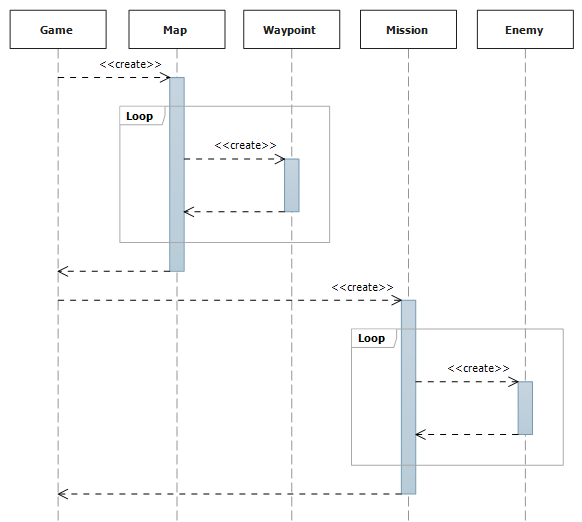
\includegraphics[width=15cm]{images/ch04/init.png}
\caption{Inicializálás. Betölti a mapet és a missiont.}
\label{fig:starting_game}
\end{center}
\end{figure}

\begin{figure}[H]
\begin{center}
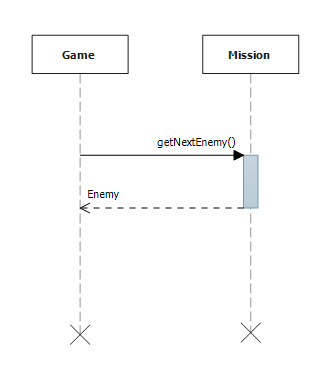
\includegraphics[width=8cm]{images/scheduling_enemies.png}
\caption{Ellenségek ütemezése.}
\label{fig:scheduling_enemies}
\end{center}
\end{figure}

\begin{figure}[H]
\begin{center}
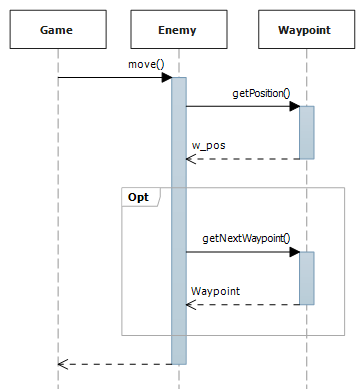
\includegraphics[width=10cm]{images/ch04/move_enemy.png}
\caption{Ellenség mozgatása. Ha elérte a waypointot lekéri a következőt.}
\label{fig:moving_enemy}
\end{center}
\end{figure}

\begin{figure}[H]
\begin{center}
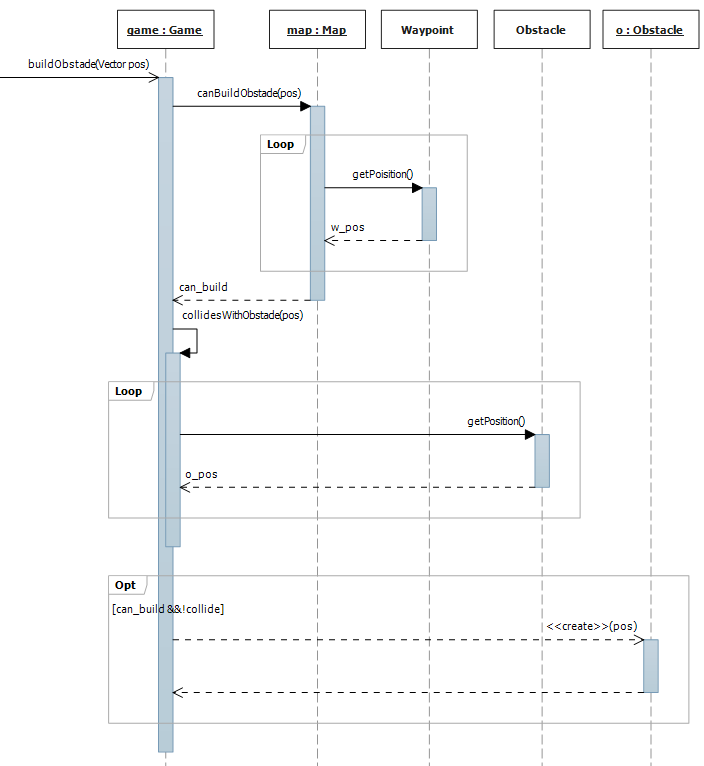
\includegraphics[width=480px]{images/ch04/build_obstacle.png}
\caption{Akadály építése. Megnézi, hogy szabad-e a helyre építeni, ha szabad épít.}
\label{fig:building_obstacle}
\end{center}
\end{figure}

\begin{figure}[H]
\begin{center}
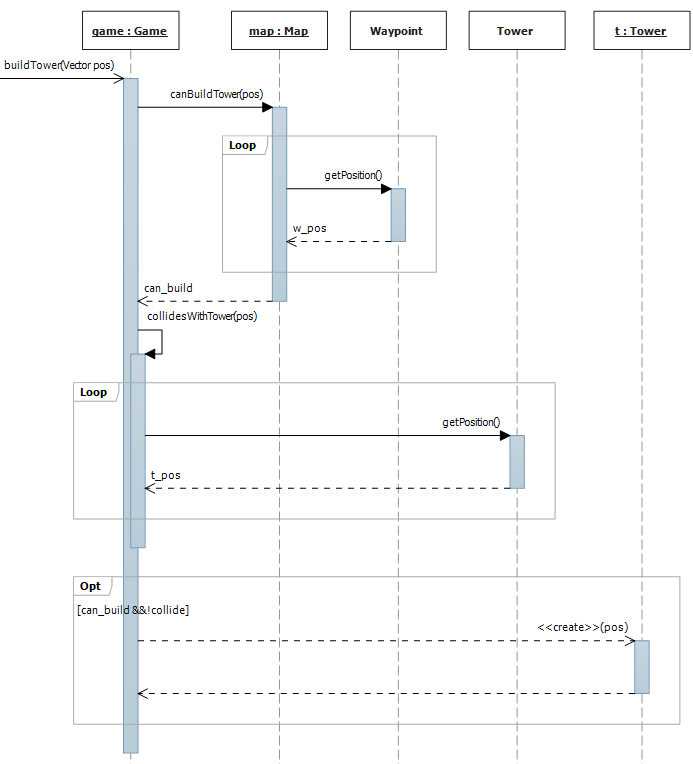
\includegraphics[width=480px]{images/ch04/build_tower.png}
\caption{Torony építése. Megnézi, hogy szabad-e a helyre építeni, ha szabad épít.}
\label{fig:building_tower}
\end{center}
\end{figure}

\begin{figure}[H]
\begin{center}
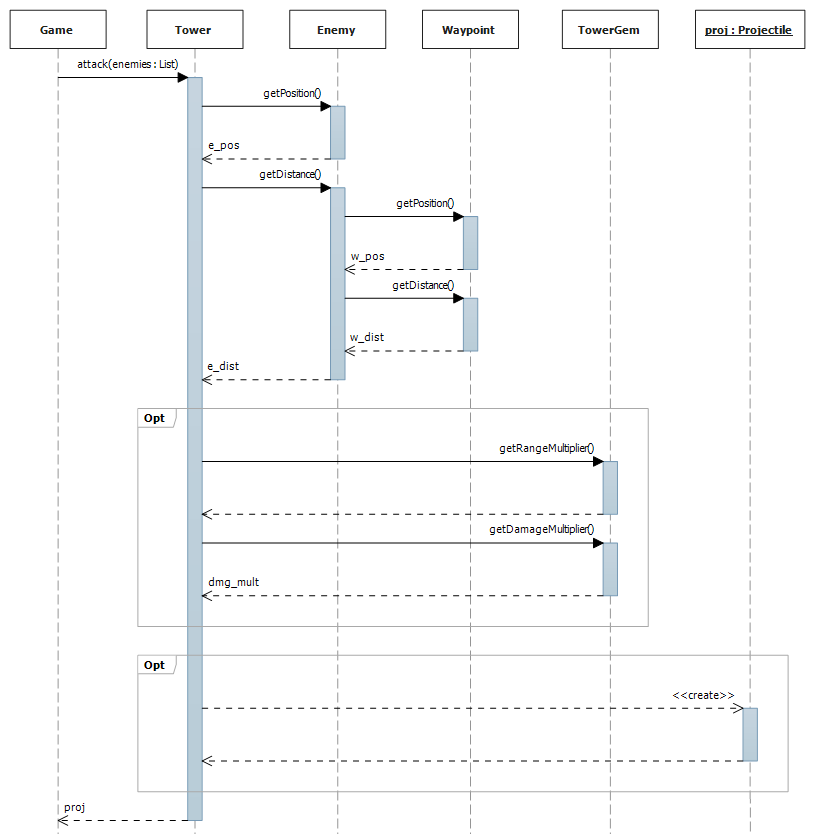
\includegraphics[width=17cm]{images/ch04/enemy_attack.png}
\caption{Ellenségek támadása. Minden ellenségre megnézi mennyire van távol a céltól és a legelsőre lő.}
\label{fig:tower_firing}
\end{center}
\end{figure}

\begin{figure}[H]
\begin{center}
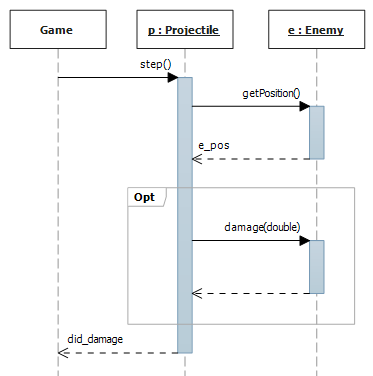
\includegraphics{images/ch04/projectile_step.png}
\caption{Lövedék léptetése.}
\label{fig:adding_gem}
\end{center}
\end{figure}

\begin{figure}[H]
\begin{center}
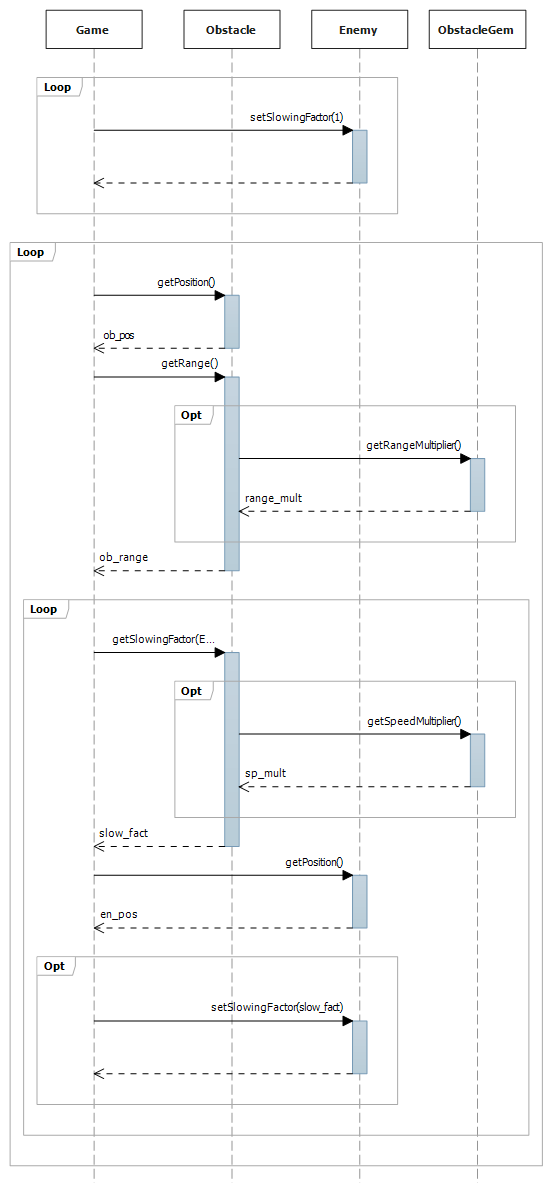
\includegraphics[width=14cm]{images/ch04/slow_enemy.png}
\caption{Minden akadály megnézi minden ellenségre, hogy a hatókörében van-e, ha igen lelassítja őket.}
\label{fig:adding_gem}
\end{center}
\end{figure}

\begin{figure}[H]
\begin{center}
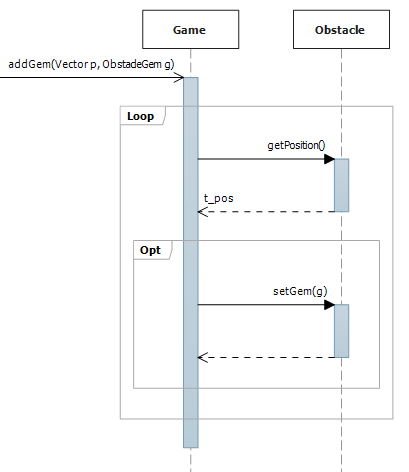
\includegraphics[width=92mm]{images/ch04/add_gem_obstacle.png}
\caption{Varázskő feltétele akadályra.}
\label{fig:adding_gem}

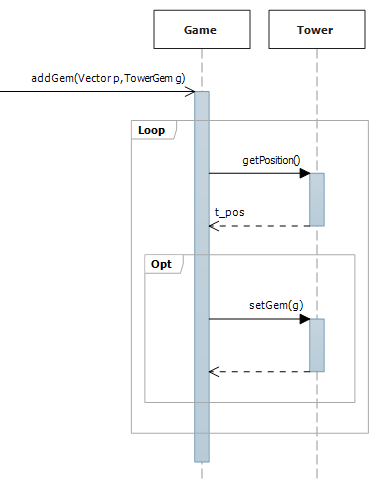
\includegraphics[width=92mm]{images/ch04/add_gem_tower.png}
\caption{Varázskő feltétele toronyra.}
\label{fig:adding_gem}
\end{center}
\end{figure}

\begin{figure}[H]
\begin{center}
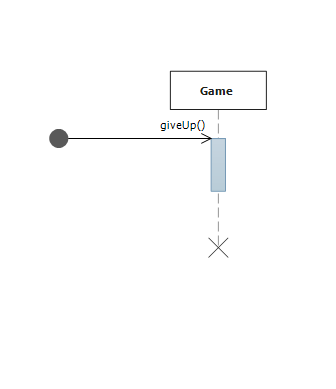
\includegraphics{images/giving_up.png}
\caption{Feladás.}
\label{fig:giving_up}
\end{center}
\end{figure}


\pagebreak
\section{State-chartok}

\begin{figure}[H]
\begin{center}
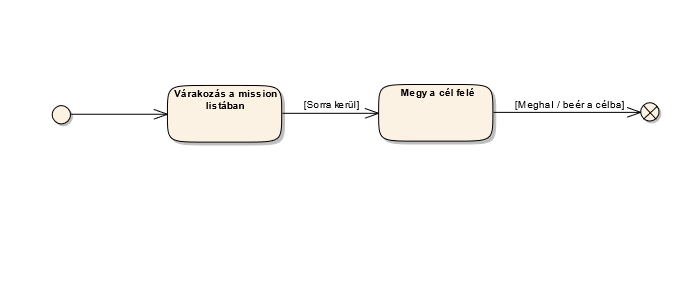
\includegraphics[width=15cm]{images/ch04/enemy_state.png}
\caption{Egy ellenség állapotdiagramja}
\label{fig:enemy_state}
\end{center}
\end{figure}

\begin{figure}[H]
\begin{center}
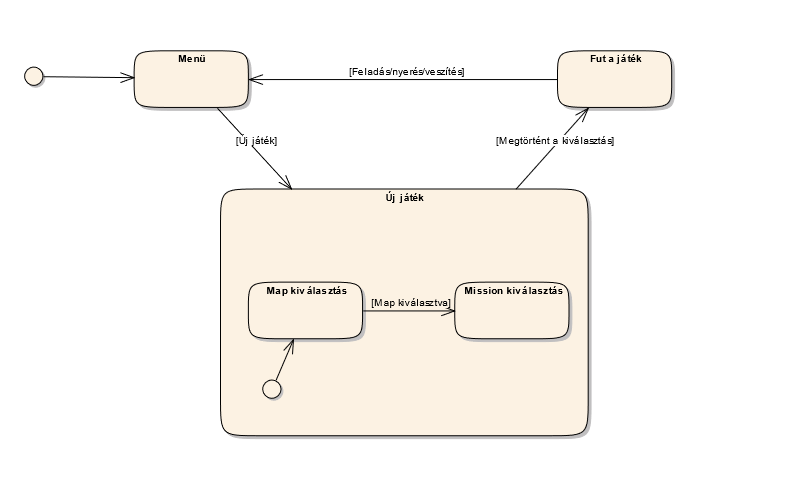
\includegraphics[width=15cm]{images/ch04/game_state.png}
\caption{A játék állapotdiagramja}
\label{fig:game_state}
\end{center}
\end{figure}

\begin{figure}[H]
\begin{center}
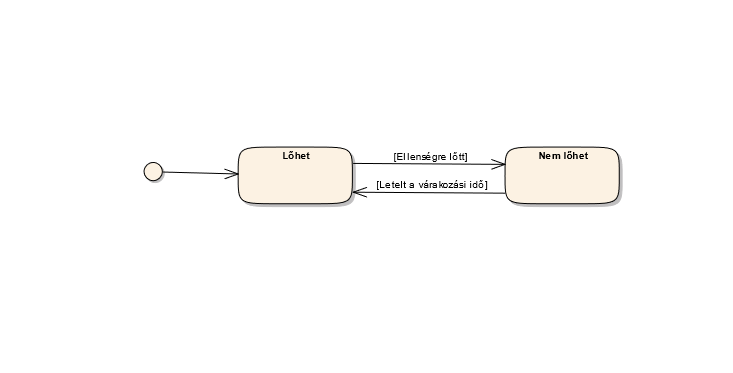
\includegraphics[width=15cm]{images/ch04/tower_state.png}
\caption{Egy torony állapotdiagramja}
\label{fig:tower_state}
\end{center}
\end{figure}

